\section{Approach} \label{approach}

In this section we discribe the general flow that a piece of software would go through in our proposed setup, shown by Figure~\ref{deeplearningflow}. For the sake of simplicity and readability we will use Java as the example programming language during discussion for the rest of the paper. However, it should be noted that these ideas can be applied to any programming language with some modification.

\begin{figure}
   \centering
   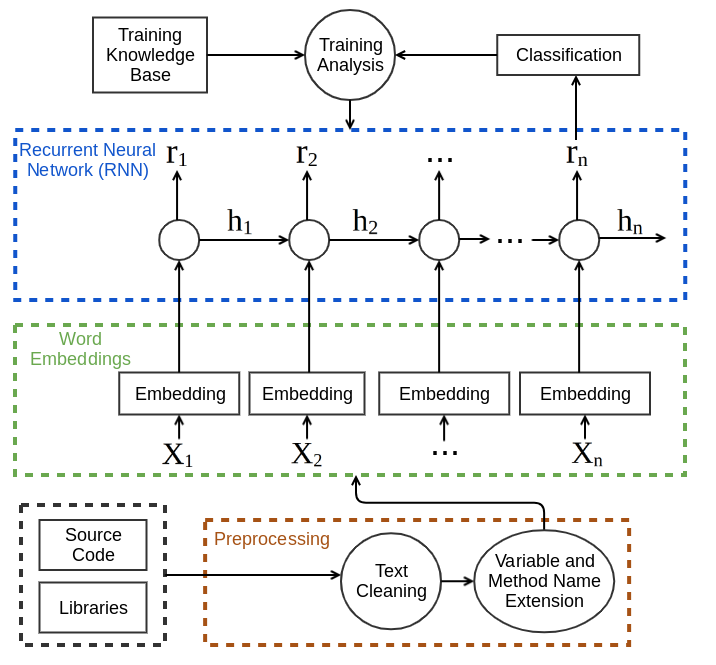
\includegraphics[scale=.36]{figures/deeplearningflow.png}
   \caption{Flow of Deep Learning Analysis}
   \vspace{-.6cm}
   \label{deeplearningflow}
\end{figure}

\subsection{Preprocessing}

The source code will need to be preprocessed before being used as input to Word2Vec. Preprocessing is represented by the brown section in Figure~\ref{deeplearningflow}. The initial preprocessing step is basic text cleaning. This includes the removal of all unnecessary white space, comments, and some punctuation. Most punctuation is kept as much of it is necessary in determining the proper structure of the source code. Some of it will also be necessary for the modified Word2Vec algorithm to perform properly.

The main preprocessing step is the identification of the scope of variables and methods. For example, given a particular class in Java, a class variable can have the same name as a local variable. Similarly, two different classes may have the same method name. This is not a problem for natural language as every word in a natural language is unique. While having variables and methods with the same name is legal in Java (within certain rules), it can heavily skew the values of the word embeddings as all variables and methods with the same name will be mapped to the same word embedding. To account for this problem, we propose to extend all variable and method names with the class and method they belong to based on their scope. For example, given the Java class \textit{String}, its method \textit{charAt} will be extended to \textit{String.charAt}, and the local variable \textit{index} in the method \textit{charAt} will be extended to \textit{String.charAt.index}. This will ensure that all variable and method names are mapped to their own word embeddings. However, this causes a new problem. If variable and method names are extended to be specific to the class they are defined in, then when analyzing new software there will be no word embeddings for any newly defined variables and methods. To remedy this, new software must first be input through Word2Vec to produce the new necessary word embeddings before being used as input to a deep learning model.

We acknowledge that there are other possible preprocessing steps that can be taken, but we do not consider these at this time. For example, in Java it is legal to overload methods (that is, have different definitions and parameter lists for the same method name). We consider overloading the same as a word in natural language having multiple definitions. While the method is somewhat ambiguated, we believe it will not ambiguate enough to drastically change the results of a deep learning analysis.

\subsection{Modified Word2Vec}

As described earlier, Word2Vec uses a window size to determine the context of a word. This works fairly well for natural language processing because each word has a general predefined meaning and the syntax of a sentence does not allow for complex syntactic structures such as decision or loop statements. So a window size that only scans for context a bit before and after a word is able to determine a relative semantic meaning to other words. However, in source code, variables and methods are defined within their class (and not always before they are used in the case of methods) and there are more complex syntactic structures. This seems to imply that a simple window size that scans before and after a word will not be sufficient in determining proper word embeddings for source code.

Word embeddings are represented by the green section in Figure~\ref{deeplearningflow}. To modify Word2Vec to process source code more effectively, we will need to separate ``keywords'' (which includes keywords, punctuation, and operands) from ``constructed words'' (which includes class, method, and variable names) as keywords are usually handled by the compiler and are not explicitly defined in a library, unlike constructed words. We further divide keywords into two categories, those that have a syntactic structure associated with them and those that do not. Such keywords that have syntactic structures are \textit{if-else}, \textit{while}, \textit{for}, etc. These keywords derive most of their meaning from their syntactic structure. Therefore, instead of using a window size, Word2Vec will consider everything that is a part of the structure as context when updating the word embedding values of that keyword. For example, in the snipet \textit{for(i; i $<$ 10; i++)\{ System.out.println(i); \}} everything between the parenthesis after the \textit{for} and before the \textit{\{} will be considered as context for the keyword \textit{for}. It is important to note that we do not consider the statement within the loop structure (\textit{System.out.println(i);}) as part of the context for the keyword \textit{for}, as the statements within keyword syntactic structures do not usually have a direct relation on the meaning of the structure (and the keyword associated with that structure). For the keywords that do not have a syntactic structure (\textit{break}, \textit{+}, \textit{\&\&}, etc.), only context before and after the word is available to derive meaning. Therefore, Word2Vec will be used normally with a window size for these keywords.

A constructed word's embedding will use context in two separate ways. The first, and most important, is that word's definition. When a constructed word is defined, the entire definition is used as context for Word2Vec. For example, for a Java class everything in the entire class is used as context; for a method, the method signature and entire definition will be used as context; for a variable, any assignment performed on it will be used as context. The second type of context will come from the constructed word's usage in code. In this case, Word2Vec will be used normally with a window size to capture code surrounding the word as context.

\subsection{Deep Learning}

Once preprocessing and word embeddings have been completed, the source code is ready to be analyzed by a neural network, represented in the blue section in Figure~\ref{deeplearningflow}. The network we will use is an RNN. This is appropriate since the current state of code at any time is dependent on what statements have been executed before it. Starting in the main method, for each word in the code, the embedding associated with that word will be used as input to the next step in the RNN.

After all words in the source code have been processed, the final output can be used to determine whatever the RNN is attempting to learn. In Figure~\ref{deeplearningflow}, a general example for the final steps to determine mappings is shown. The final output from the RNN is transformed using softmax to classify the mapping that is most likely associated with the input code. During training, the classification determined by the RNN is analyzed against the ground truth, represented by the training knowledge base. For any incorrect classifications made by the RNN, a loss is determined which is then used to update the RNN weights through backpropagation. This should result in better classifications in the future.

